\documentclass{beamer}
% Use DS9 global theme
\usepackage{../../../shared/templates/ds9_theme}

% Title page configuration
\title[Unit 1 Review]{PHYS11 CH123:}
\subtitle{Test Prep}
\author[Mr. Gullo]{Mr. Gullo}
\date[Oct 2024]{October 2024}

% Table of contents at the beginning of each section
\AtBeginSection[]
{
  \begin{frame}
    \frametitle{Table of Contents}
    \tableofcontents[currentsection]
  \end{frame}
}


\begin{document}

\frame{\titlepage}

\section{Introduction}

\begin{frame}
\frametitle{Introduction}
\begin{itemize}
    \item This presentation covers key concepts and problem-solving techniques for your upcoming physics test
    \item We'll review problems from three chapters:
    \begin{itemize}
        \item Chapter 1: Unit Conversion and Estimation
        \item Chapter 2: Frames of Reference and Displacement
        \item Chapter 3: Kinematics and Motion
    \end{itemize}
    \item Each problem will be presented with a step-by-step solution
    \item Focus on understanding the concepts and problem-solving approaches
\end{itemize}
\end{frame}

\section{Chapter 1: Unit Conversion and Estimation}

\begin{frame}
\frametitle{Chapter 1: Problem 30}
A generation is about one-third of a lifetime. Approximately how many generations have passed since the year 0 AD?
\end{frame}

\begin{frame}
\frametitle{Chapter 1: Problem 30 - Solution}
Solution:
\begin{equation*}
\text{history} \cdot \frac{10^{11} \text{ s}}{\text{history}} \cdot \frac{1 \text{ generation}}{1/3 \text{ lifetime}} \cdot \frac{0.5 \text{ lifetime}}{10^{9} \text{ s}} = \underline{150 \text{ generations}}
\end{equation*}
\end{frame}

\begin{frame}
\frametitle{Chapter 1: Problem 30 - Explanation}
Explanation:
\begin{enumerate}
    \item Start with the total time since 0 AD (history)
    \item Convert this time to seconds: $\frac{10^{11} \text{ s}}{\text{history}}$
    \item Convert seconds to lifetimes: $\frac{0.5 \text{ lifetime}}{10^{9} \text{ s}}$
    \item Convert lifetimes to generations: $\frac{1 \text{ generation}}{1/3 \text{ lifetime}}$
    \item Multiply all these factors together
    \item This simplifies to 150 generations
\end{enumerate}
Key concept: Unit conversion and fraction multiplication
\end{frame}

\section{Chapter 2: Frames of Reference and Displacement}

\begin{frame}
\frametitle{Chapter 2: Problem 28}
Suppose a train is moving along a track. Is there a single, correct reference frame from which to describe the train's motion?

A. Yes, there is a single, correct frame of reference because motion is a relative term.\\
B. Yes, there is a single, correct frame of reference which is in terms of Earth's position.\\
C. No, there is not a single, correct frame of reference because motion is a relative term.\\
D. No, there is not a single, correct frame of reference because motion is independent of frame of reference.
\end{frame}

\begin{frame}
\frametitle{Chapter 2: Problem 28 - Solution}
Solution: The correct answer is \textbf{C}. No, there is not a single correct frame of reference because motion is a relative term.
\begin{figure}
    \centering
    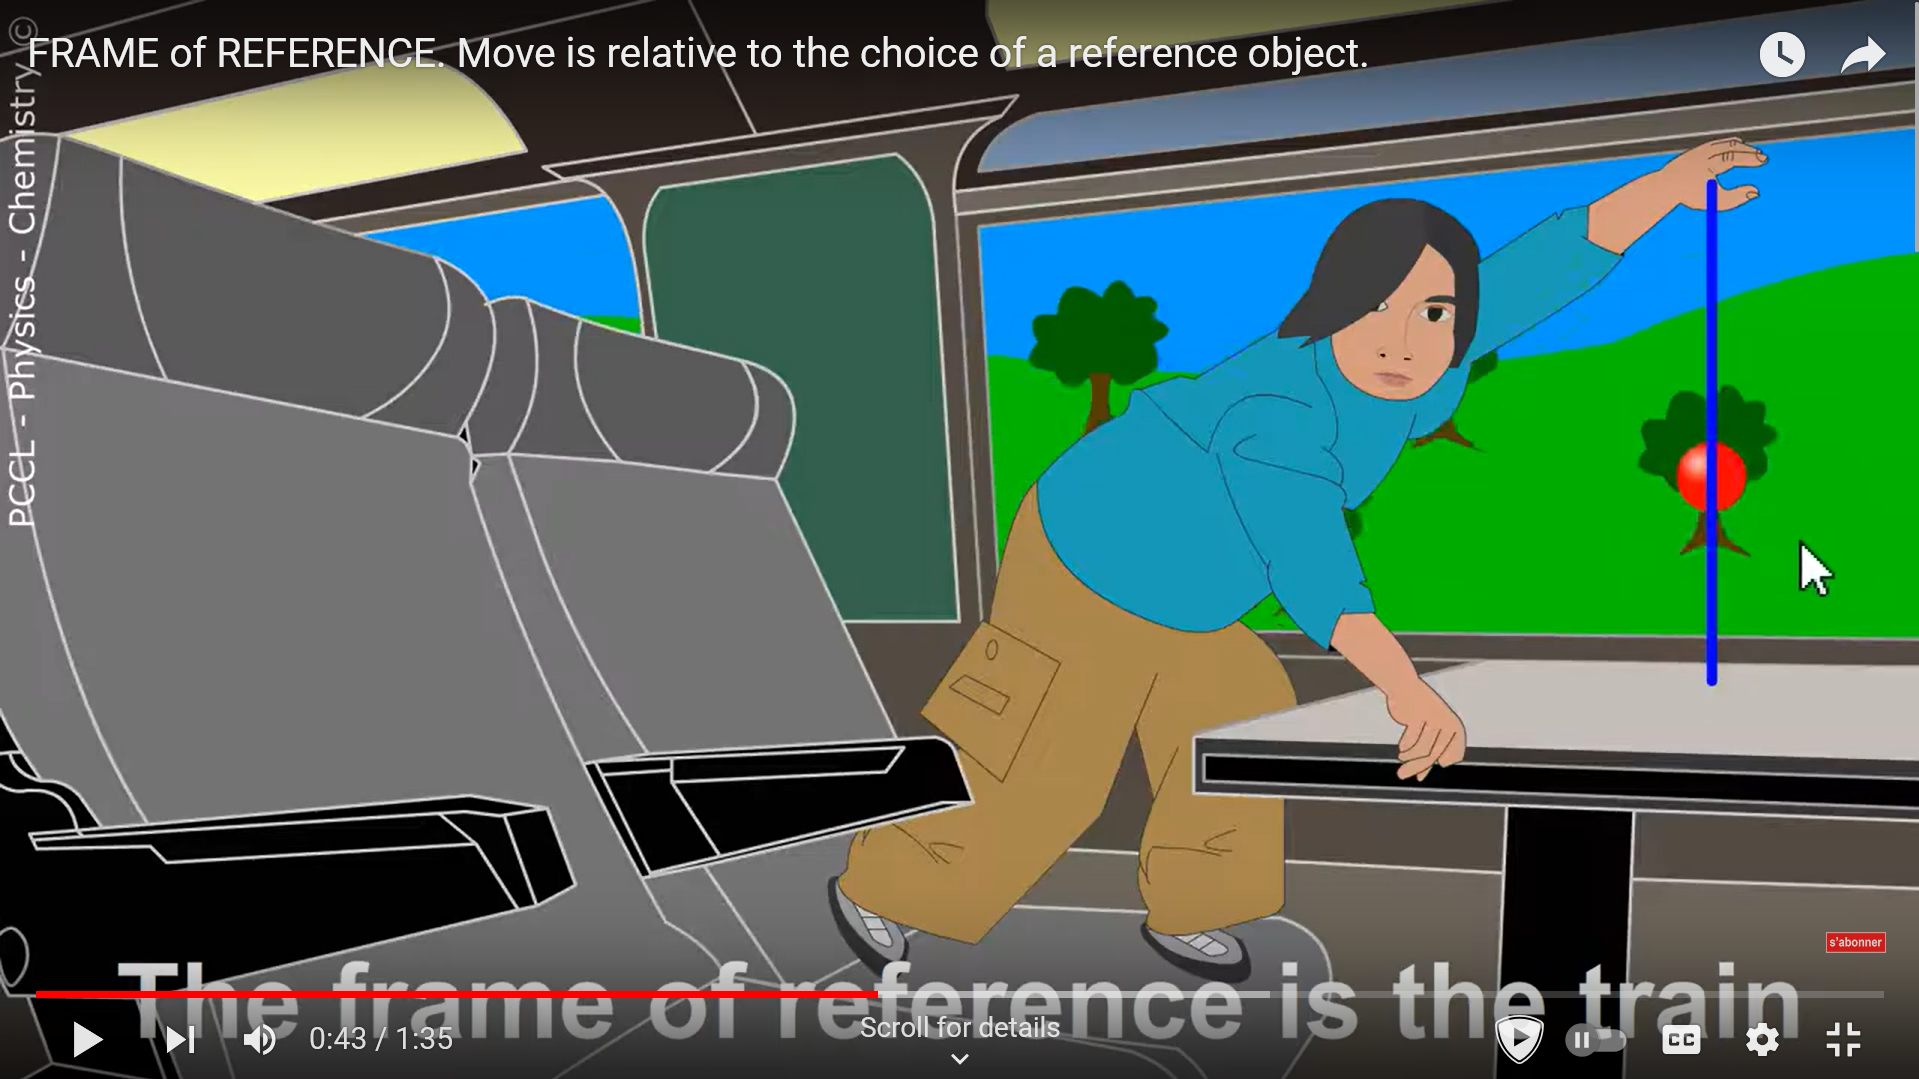
\includegraphics[width=0.5\linewidth]{phys11-motion-reference_frames_example1.png}
\end{figure}
\begin{figure}
    \centering
    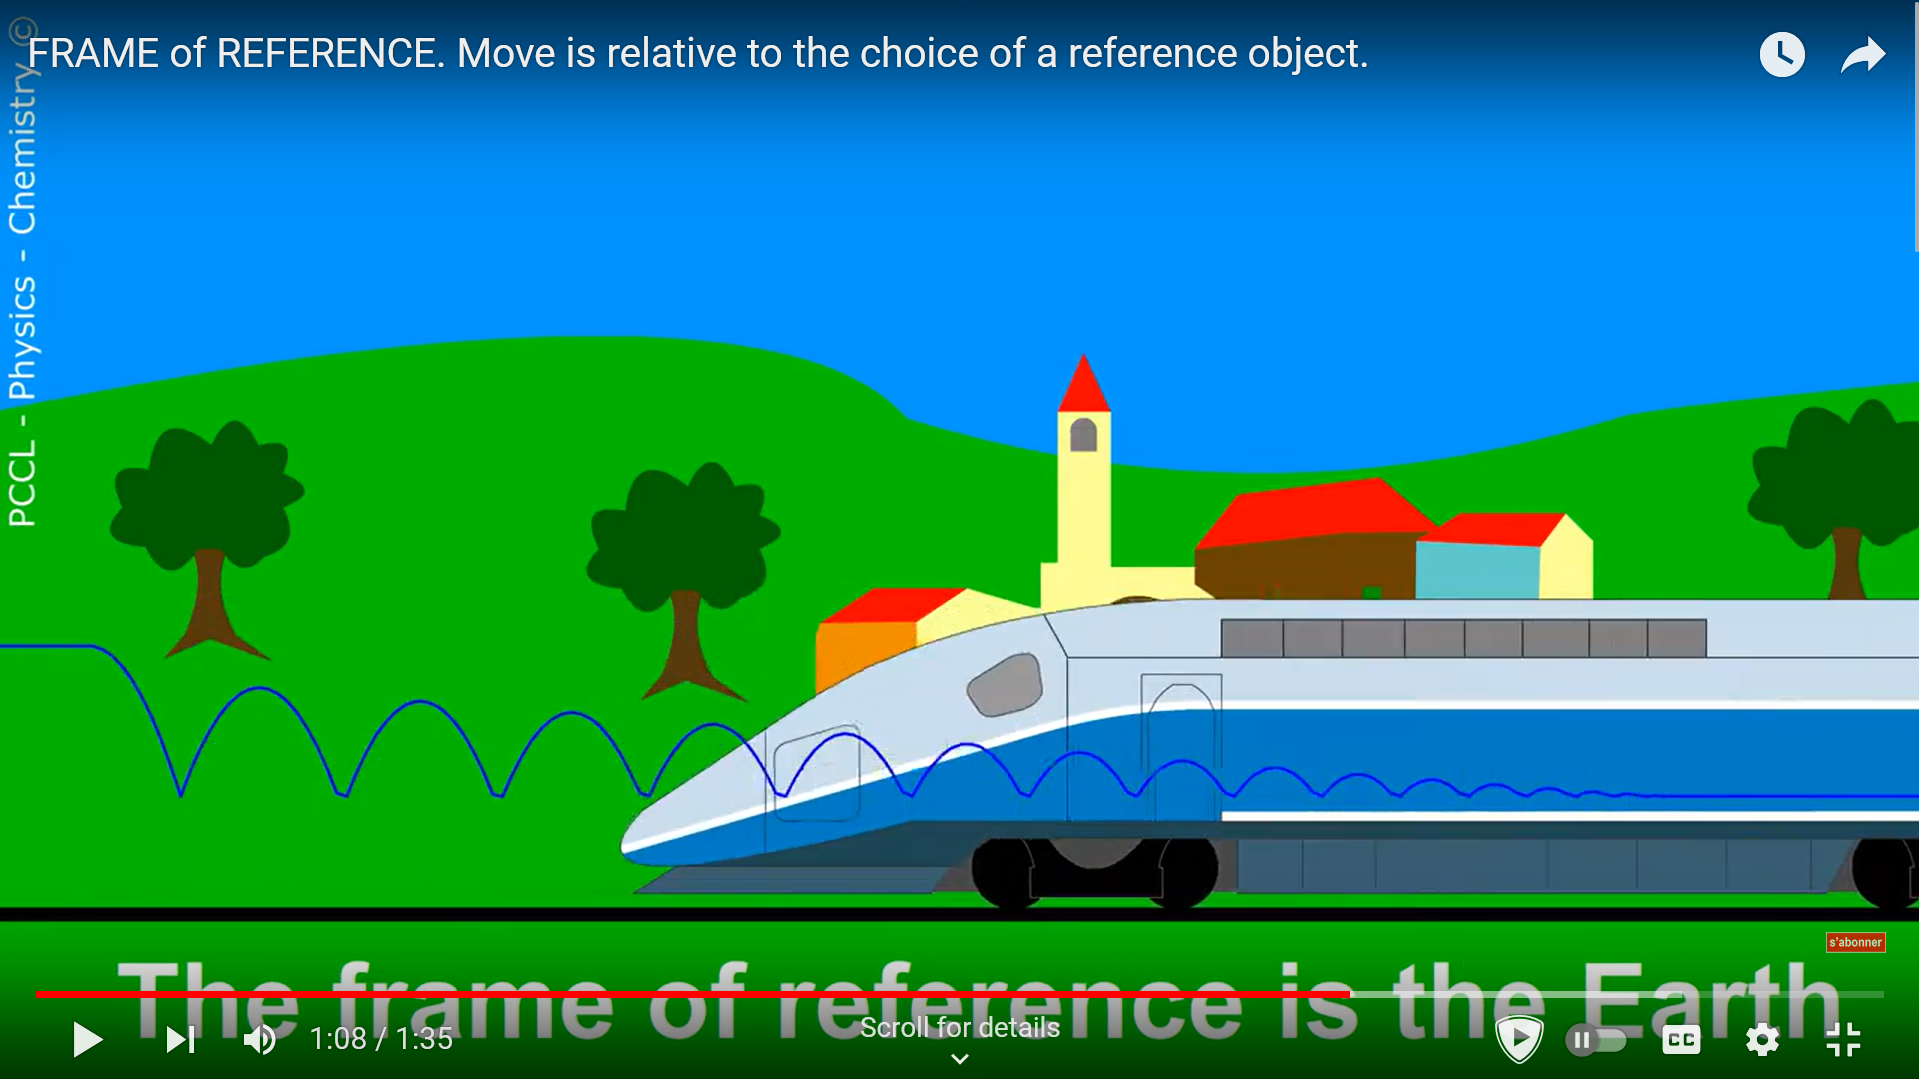
\includegraphics[width=0.5\linewidth]{phys11-motion-reference_frames_example2.png}
\end{figure}
\end{frame}


\begin{frame}
\frametitle{Chapter 2: Problem 28 - Solution}
Solution: The correct answer is \textbf{C}. No, there is not a single correct frame of reference because motion is a relative term.
Explanation:
\begin{itemize}
\item Option C is correct: Motion depends on what you compare it to (relative motion).
\item Option D is incorrect: It wrongly states that motion doesn't change with perspective.
\item Examples:
\begin{itemize}
\item On the train: Train seems still, landscape moves.
\item On the platform: Train moves, platform seems still.
\item In a car alongside: Train might seem to move slowly.
\end{itemize}
\item This illustrates the principle of relativity in physics: motion description depends on the chosen reference frame.
\end{itemize}
\end{frame}
\begin{frame}
\frametitle{Chapter 2: Problem 28 - Explanation}
Explanation:
\begin{itemize}
    \item Motion is relative: The movement of an object can be described differently depending on the observer's frame of reference
    \item Multiple valid frames: For a moving train, we could describe its motion relative to the ground, a passenger inside the train, or even another moving object
    \item Each frame is correct: The motion described from each of these perspectives would be correct for that particular frame of reference
    \item No absolute frame: There isn't a single, universally "correct" frame of reference that takes precedence over others
\end{itemize}
Key concept: Relativity of motion and frames of reference
\end{frame}

\begin{frame}
\frametitle{Chapter 2: Problem 51}
Calculate that object's net displacement over the time shown.
\begin{figure}
    \centering
    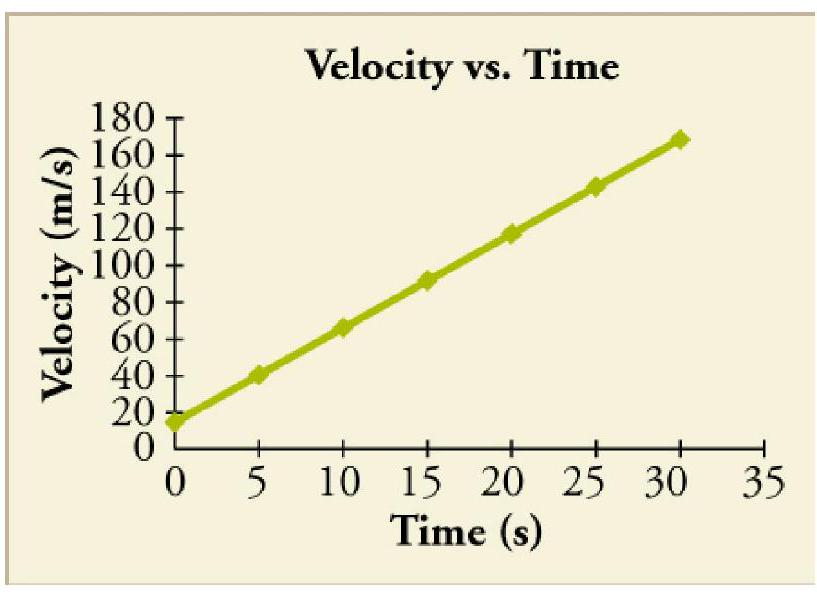
\includegraphics[width=0.5\linewidth]{2024_09_22_d75bb9ada91612339d1ag-12.jpg}
\end{figure}

A. 540 m
B. 2,520 m
C. 2,790 m
D. 5,040 m
\end{frame}

\begin{frame}
\frametitle{Chapter 2: Problem 51 - Solution}
Solution: The correct answer is \textbf{C}. The net displacement is 2,790 m.

Calculation:
\begin{itemize}
    \item Area of rectangle: $18 \text{ m/s} \cdot 30 \text{ s} = 540 \text{ m}$
    \item Area of triangle: $\frac{1}{2} \cdot 150 \text{ m/s} \cdot 30 \text{ s} = 2,250 \text{ m}$
    \item Total area: $540 \text{ m} + 2,250 \text{ m} = 2,790 \text{ m}$
\end{itemize}
\end{frame}

\begin{frame}
\frametitle{Chapter 2: Problem 51 - Explanation}
Explanation:
\begin{enumerate}
    \item Identify the shape: The area under the line consists of a rectangle and a triangle
    \item Calculate the area of the rectangle: $18 \text{ m/s} \cdot 30 \text{ s} = 540 \text{ m}$
    \item Calculate the area of the triangle: $\frac{1}{2} \cdot 150 \text{ m/s} \cdot 30 \text{ s} = 2,250 \text{ m}$
    \item Sum the areas: $540 \text{ m} + 2,250 \text{ m} = 2,790 \text{ m}$
\end{enumerate}
Key concept: In a velocity-time graph, the area under the curve represents displacement
\end{frame}

\section{Chapter 3: Kinematics and Motion}

\begin{frame}
\frametitle{Chapter 3: Problem 32}
You throw a ball straight up with an initial velocity of 15.0 m/s. It passes a tree branch on the way up at a height of 7.00 m. How much additional time will pass before the ball passes the tree branch on the way back down?

A. 0.574 s
B. 0.956 s
C. 1.53 s
D. 1.91 s
\end{frame}

\begin{frame}
\frametitle{Chapter 3: Problem 32 - Solution Part 1}
Solution: The correct answer is \textbf{D}. 1.91 s

Step 1: Find the velocity at the branch
\begin{align*}
v^2 &= v_0^2 + 2a(x-x_0) \\
v &= \sqrt{v_0^2 + 2a(x-x_0)} \\
v &= \sqrt{(15.0 \text{ m/s})^2 + 2(-9.8 \text{ m/s}^2)(7 \text{ m} - 0 \text{ m})} \\
v &= 9.37 \text{ m/s}
\end{align*}
\end{frame}

\begin{frame}
\frametitle{Chapter 3: Problem 32 - Solution Part 2}
Step 2: Find the time from the branch to the top
\begin{align*}
v &= v_0 + at \\
t_1 &= \frac{v - v_0}{a} = \frac{0 \text{ m/s} - 9.37 \text{ m/s}}{-9.8 \text{ m/s}^2} = 0.956 \text{ s}
\end{align*}

Step 3: Double the time for total up and down
\begin{equation*}
t = 2t_1 = 2(0.956 \text{ s}) = 1.91 \text{ s}
\end{equation*}
\end{frame}

\begin{frame}
\frametitle{Chapter 3: Problem 32 - Explanation}
Explanation:
\begin{enumerate}
    \item Use $v^2 = v_0^2 + 2a(x-x_0)$ to find velocity at the branch
    \item Use $v = v_0 + at$ to find time from branch to top
    \item Double this time for total time up and down
\end{enumerate}
Key concepts:
\begin{itemize}
    \item Kinematic equations for constant acceleration
    \item Symmetry of motion under constant acceleration
    \item Negative acceleration for upward motion
\end{itemize}
\end{frame}

\section{Conclusion}

\begin{frame}
\frametitle{Conclusion}
\begin{itemize}
    \item We've covered key problems from three important chapters:
    \begin{itemize}
        \item Unit conversion and estimation
        \item Frames of reference and displacement
        \item Kinematics and motion
    \end{itemize}
    \item Focus on understanding the concepts behind each problem
    \item Practice applying these problem-solving techniques
    \item Remember to identify given information, choose appropriate equations, and check units
    \item Good luck on your upcoming test!
\end{itemize}
\end{frame}

\end{document}
